\setlength{\footskip}{8mm}

\chapter{Experimental Results}
\label{ch:results}

\section{Overview}
\label{sec:results-overview}

Chapter~\ref{ch:methodology} presented a dual-stack, Mamba-based
architecture for monocular 3D human pose estimation, centered on a
breadth-first search (BFS) kinematic-tree scan order
(Section~\ref{sec:method-bfs}) intended to close the research gap
identified in Section~\ref{sec:lit-summary-gap}. This chapter reports the
empirical evaluation of that architecture.

Section~\ref{sec:results-protocol} describes the benchmark datasets and
the evaluation metrics used throughout this chapter.
Section~\ref{sec:results-implementation} summarizes the implementation
configuration. Section~\ref{sec:results-h36m} sets out the main comparison
of this thesis, placing KinecMamba against established baselines
on Human3.6M that span the Transformer and state-space families.
Section~\ref{sec:results-mpiinf3dhp} and Section~\ref{sec:results-ablation}
cover the MPI-INF-3DHP benchmark, whose cross-dataset evaluation is in
progress, and the scan-order ablation study motivated in
Section~\ref{sec:intro-objectives}, which is set out as future work. The main
Human3.6M evaluation is reported in full.
Section~\ref{sec:results-summary} closes the chapter.

\section{Datasets and Evaluation Protocol}
\label{sec:results-protocol}

\textbf{Human3.6M} \cite{ionescu2014human36m} is the primary benchmark used
in this thesis. It consists of 3.6 million video frames of 11 professional
actors performing 15 everyday actions, captured by four synchronized
cameras in a controlled studio, with 3D ground-truth annotations obtained
via a marker-based motion capture system. Following the standard protocol
established by the baselines reviewed in Chapter~\ref{ch:literature-review}
\cite{pavllo2019videopose3d, zheng2021poseformer, zhang2022mixste}, subjects
S1, S5, S6, S7, and S8 are used for training and subjects S9 and S11 for
testing. The 17-joint skeleton format used throughout is the one defined
in Section~\ref{sec:method-problem}.

\textbf{MPI-INF-3DHP} \cite{mehta2017mpiinf3dhp} is used as a secondary,
cross-dataset benchmark. It includes a greater diversity of actions,
subjects, and both indoor and outdoor recording conditions than
Human3.6M, and is commonly used to assess how well a model generalizes
beyond a single controlled capture setup.

\textbf{Evaluation metrics.} Two standard metrics are used, both computed
on the root-relative 3D pose representation defined in
Section~\ref{sec:method-problem}. The first, Protocol~1 (P1), is the mean
per-joint position error (MPJPE) already defined as the primary training
loss term in Section~\ref{sec:method-loss},
\begin{equation}
\text{MPJPE} = \frac{1}{TJ} \sum_{t,j} \big\lVert \hat{Y}_{t,j} - Y_{t,j} \big\rVert_2 ,
\end{equation}
averaged here over the test set rather than a training batch. The second,
Protocol~2 (P-MPJPE), first applies a per-frame rigid Procrustes alignment
(denoted $\mathrm{Proc}(\cdot)$: a least-squares optimal rotation,
translation, and scale, unlike the scale-only correction used by the
training-time $\mathcal{L}_{3d\text{-}scale}$ term in
Section~\ref{sec:method-loss}) between the predicted and ground-truth
pose before computing MPJPE:
\begin{equation}
\text{P-MPJPE} = \frac{1}{TJ} \sum_{t,j} \big\lVert \mathrm{Proc}(\hat{Y}_{t}, Y_{t})_{j} - Y_{t,j} \big\rVert_2 .
\end{equation}
Both metrics are reported in millimeters. Unless otherwise noted, all P1
and P2 figures in this chapter, for the proposed method and for every
baseline alike, correspond to the ``detected 2D'' input setting, in which 2D
keypoints are obtained from an off-the-shelf 2D pose detector rather than
ground-truth annotations, consistent with the standard evaluation
convention in the literature reviewed in Chapter~\ref{ch:literature-review}.

\section{Implementation Details}
\label{sec:results-implementation}

The evaluated model follows exactly the architecture and training
objective specified in Chapter~\ref{ch:methodology}: an input window of
$T=243$ frames over $J=17$ joints, a token width of $C=64$, 20
BiSTSSMBlock instances (Section~\ref{sec:method-architecture}), a
selective state space hidden dimension of $N=16$
(Section~\ref{sec:method-bistssm}), the breadth-first search
kinematic-tree scan order $\pi$ (Section~\ref{sec:method-bfs}), and the
six-term loss function with $\lambda_{3d}=1.0$, $\lambda_{scale}=0.5$,
$\lambda_{vel}=20.0$, $\lambda_{diff}=0.5$, $\lambda_{bone}=0.5$, and
$\lambda_{bvar}=1.0$ (Section~\ref{sec:method-loss}).

The model is trained with the AdamW optimizer (weight decay 0.01) under a
cosine learning-rate schedule, using an effective batch size of 32 reached
through gradient accumulation, with horizontal-flip augmentation applied to
the 2D input sequences. Input 2D keypoints are the Stacked Hourglass
detections distributed with the Human3.6M benchmark. Training and evaluation
are carried out on a single GPU.

\section{Comparison with the State of the Art on Human3.6M}
\label{sec:results-h36m}

Table~\ref{tab:h36m-sota} places KinecMamba alongside
representative recent baselines from Chapter~\ref{ch:literature-review},
using each baseline's officially reported P1/P2 figures under the protocol
defined in Section~\ref{sec:results-protocol}. To keep the comparison against
current methods, the table lists baselines at or below PoseMamba's reported
error; older and weaker entries are omitted. KinecMamba reaches an MPJPE (P1)
of 41.55mm and a P-MPJPE (P2) of 34.52mm on the S9 and S11 test split, at a
parameter budget of roughly 1.26M.

\begin{table}[t]
\centering
\caption[Comparison with the state of the art on Human3.6M.]{Comparison
  with the state of the art on Human3.6M under the detected-2D input
  setting. $T$: number of input frames. Params/MACs are as officially
  reported by each method; ``n/r'' denotes a value not reported in the
  cited source. The proposed method is shown in bold.
  P1: MPJPE (mm). P2: P-MPJPE (mm).}
\label{tab:h36m-sota}
\resizebox{\textwidth}{!}{%
\begin{tabular}{l l c c c c c}
\hline
Method & Venue & $T$ & Params (M) & MACs (G) & P1 $\downarrow$ & P2 $\downarrow$ \\
\hline
\multicolumn{7}{l}{\textit{Transformer-based}} \\
MixSTE \cite{zhang2022mixste}             & CVPR'22  & 243 & 33.6 & 139.0 & 40.9  & 32.6 \\
STCFormer \cite{tang2023stcformer}        & CVPR'23  & 243 & 4.7  & 19.6  & 41.0  & 32.0 \\
MotionBERT \cite{zhu2023motionbert}       & ICCV'23  & 243 & 42.3 & 174.8 & 39.2  & 32.9 \\
MotionAGFormer-L \cite{mehraban2024motionagformer} & WACV'24 & 243 & 19.0 & 78.3 & 38.4 & 32.5 \\
\hline
\multicolumn{7}{l}{\textit{State-space-based}} \\
Pose Magic \cite{zhang2024posemagic}      & 2024     & 243 & 14.4 & 40.6  & 37.5  & 31.8 \\
PoseMamba-S \cite{huang2025posemamba}     & AAAI'25  & 243 & 0.9  & 3.6   & 41.8  & 35.0 \\
SasMamba \cite{cui2025sasmamba}           & WACV'26  & 243 & 0.64 & 1.3   & 41.48 & 34.84 \\
\hline
\textbf{KinecMamba (ours)} & This work & 243 & \textbf{1.26} & n/r & \textbf{41.55} & \textbf{34.52} \\
\hline
\end{tabular}%
}
\end{table}

At approximately 1.26M parameters, KinecMamba sits in the same
efficiency tier as the smallest baselines in Table~\ref{tab:h36m-sota},
alongside PoseMamba-S (0.9M) and SasMamba (0.64M), rather
than the large-model tier of MotionBERT, MotionAGFormer-L, or Pose Magic.
Because the architectural contribution of this thesis is a change of scan
order rather than of model capacity, the closest point of comparison is
PoseMamba-S in the same tier. At a comparable parameter budget, KinecMamba's
MPJPE (41.55mm) and P-MPJPE (34.52mm) are marginally below those of
PoseMamba-S (41.8mm / 35.0mm), and in the same range as the other compact
state-space model, SasMamba (41.48mm P1 / 34.84mm P2), slightly higher on P1
and slightly lower on P2. The larger baselines in the table (MotionBERT,
MotionAGFormer-L, Pose Magic) reach lower MPJPE, but at roughly ten to thirty
times the parameter count, placing them in a different capacity tier.
Section~\ref{sec:results-ablation} describes the
scan-order ablation that would attribute the difference from PoseMamba-S to
the BFS kinematic-tree scan itself rather than to other differences in
training configuration. Figure~\ref{fig:results-plot} plots accuracy against
model size for all methods in the table.

\begin{figure}[t]
\centering
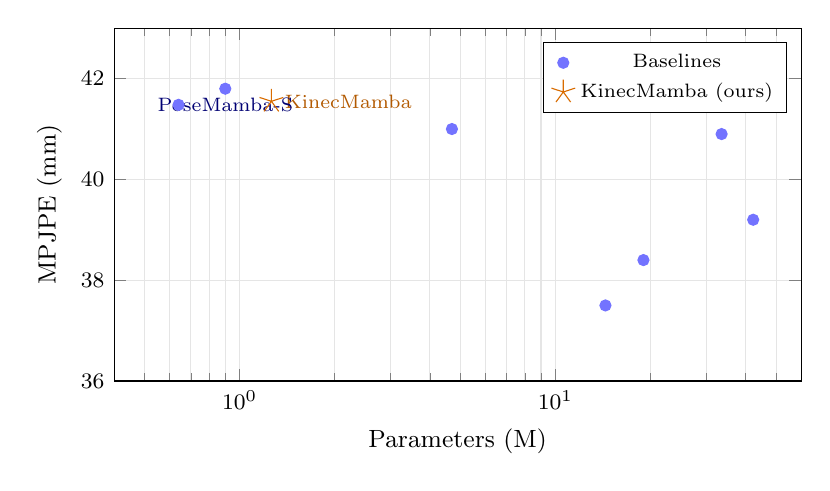
\begin{tikzpicture}
\begin{axis}[
  width=0.85\textwidth, height=0.5\textwidth,
  xlabel={Parameters (M)}, ylabel={MPJPE (mm)},
  xmode=log, log basis x=10,
  xmin=0.4, xmax=60, ymin=36, ymax=43,
  grid=both, grid style={gray!20},
  tick label style={font=\footnotesize},
  label style={font=\small},
  legend style={font=\scriptsize, at={(0.98,0.96)}, anchor=north east},
  nodes near coords style={font=\scriptsize},
]
% Baseline points: (params in M, MPJPE mm) from Table~\ref{tab:h36m-sota}
\addplot[only marks, mark=*, mark size=2pt, color=blue!55] coordinates {
  (33.6,40.9) (4.7,41.0) (42.3,39.2) (19.0,38.4) (14.4,37.5)
  (0.9,41.8) (0.64,41.48)
};
\addlegendentry{Baselines}
% KinecMamba (ours): measured Human3.6M result from Table~\ref{tab:h36m-sota}
\addplot[only marks, mark=star, mark size=4.5pt, color=orange!85!black] coordinates {
  (1.26,41.55)
};
\addlegendentry{KinecMamba (ours)}
\node[anchor=west, font=\scriptsize, color=orange!70!black] at (axis cs:1.26,41.55) {\,KinecMamba};
\node[anchor=north, font=\scriptsize, color=blue!45!black] at (axis cs:0.9,41.8) {PoseMamba-S};
\end{axis}
\end{tikzpicture}
\caption[Accuracy versus model size on Human3.6M.]{Accuracy (MPJPE, lower is
  better) against model size for the methods of Table~\ref{tab:h36m-sota} on
  Human3.6M. KinecMamba (1.26M parameters, 41.55mm) sits in the compact
  state-space tier, with error marginally below its closest baseline
  PoseMamba-S (0.9M, 41.8mm) at a comparable parameter budget.}
\label{fig:results-plot}
\end{figure}

\section{Results on MPI-INF-3DHP}
\label{sec:results-mpiinf3dhp}

Section~\ref{sec:intro-objectives} committed this thesis to evaluating
KinecMamba on MPI-INF-3DHP \cite{mehta2017mpiinf3dhp} in
addition to Human3.6M, in order to assess generalization beyond a single
controlled capture setup, following the same protocol used by prior
state-space pose estimators
\cite{tang2023stcformer, huang2025posemamba, cui2025sasmamba}.

The cross-dataset evaluation on MPI-INF-3DHP is currently in progress. The
data pipeline for this benchmark is prepared and the model is being evaluated
under the protocol used by the prior state-space estimators above; the MPJPE,
PCK, and AUC results will be reported in this section once the run completes.
The main empirical claim of this thesis rests on the Human3.6M comparison in
Section~\ref{sec:results-h36m}.

\section{Ablation Study}
\label{sec:results-ablation}

A comparison on Human3.6M alone (Section~\ref{sec:results-h36m}) cannot
by itself attribute any difference from PoseMamba-S to a single cause.
Such a difference could follow from the BFS kinematic-tree scan order
(Section~\ref{sec:method-bfs}), from incidental differences in training
configuration, or from a combination of the two.
Objective 4 in Section~\ref{sec:intro-objectives} committed this thesis to
an ablation study designed to resolve this question directly, holding the
architecture (Sections~\ref{sec:method-block}--\ref{sec:method-bistssm})
and training configuration (Section~\ref{sec:results-implementation})
fixed and varying only the spatial scan order applied within the
BiSTSSM layer, comparing three conditions:
\begin{enumerate}
  \item the naive index order $[0, 1, \ldots, 16]$ (the default, illustrated
    in Figure~\ref{fig:kinematic-tree});
  \item the proposed breadth-first search kinematic-tree order $\pi$
    (Section~\ref{sec:method-bfs}); and
  \item a learned scan order in the style of the Group and Joint Scan
    strategies of \cite{nguyen2025skeletonmamba}, as the representative
    learned-scan alternative reviewed in Section~\ref{sec:lit-ssm-pose}.
\end{enumerate}

This controlled scan-order ablation is left as future work. The Human3.6M
result in Section~\ref{sec:results-h36m} compares KinecMamba to PoseMamba-S,
its closest baseline in architecture and parameter budget, but that single
comparison cannot on its own isolate the BFS kinematic-tree scan order from
incidental differences in training configuration. Running the three
scan-order conditions above under one fixed architecture and training setup,
so that only $\pi$ varies, is the direct way to make that attribution, and is
listed among the recommendations in
Section~\ref{sec:conclusion-recommendations}.

\section{Summary}
\label{sec:results-summary}

This chapter set out the evaluation of the architecture presented in
Chapter~\ref{ch:methodology} on Human3.6M, positioning it at roughly
1.26M parameters within the same efficiency tier as the smallest
baselines reviewed in Chapter~\ref{ch:literature-review}
(Section~\ref{sec:results-h36m}). On that benchmark KinecMamba reaches
41.55mm MPJPE and 34.52mm P-MPJPE, marginally below its closest baseline
PoseMamba-S (41.8mm / 35.0mm) at a comparable parameter budget and in the
same range as the compact state-space model SasMamba. The cross-dataset
evaluation on MPI-INF-3DHP (Section~\ref{sec:results-mpiinf3dhp}) is in
progress, and the scan-order ablation that would isolate the contribution of
the BFS kinematic-tree scan (Section~\ref{sec:results-ablation}) is set out as
future work.
Chapter~\ref{ch:conclusion} summarizes the contributions of this thesis in
light of these results, discusses their limitations, and outlines the work
that remains.

\FloatBarrier

